% !TEX root = ../../../main.tex
% 来源：中学数学实验教材·第二册（几何）
% 章节：集合与简易逻辑 / 简易逻辑
% 原始文件：2.tex，行 1204-1214
% 类型：tikz
% ---
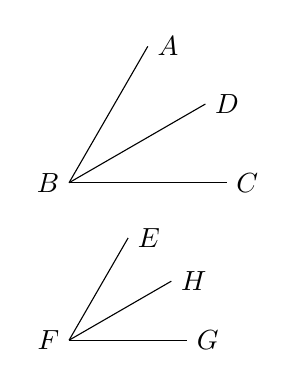
\begin{tikzpicture}[>=latex, scale=1]
      \foreach \x/\xtext in {30/D,60/A,0/C}
{
	\draw(0,0)--(\x:2)node[right]{$\xtext$};
}
\node at (0,0)[left]{$B$}; 

\draw (0,-2)node[left]{$F$}--(1.5,-2)node[right]{$G$};
\draw (0,-2)--(.75*1.732,-2+.75)node[right]{$H$};
\draw (0,-2)--(.75,-2+.75*1.732)node[right]{$E$};       
    \end{tikzpicture}
